% L7c linear regression schematic: observations, the fitted model line, and
% the residuals, labeled in the lecture's notation. The lecture writes a
% linear model as y_i = \hat{x}_i^T \theta + \epsilon_i, with augmented
% features \hat{x}_i = (x_i, 1) and estimated parameters \hat{\theta}, and
% defines the residual r_i = y_i - \hat{x}_i^T \hat{\theta}.
%
% Redrawn on October 5, 2026 after the Fall 2025 schematic, which labeled the
% residual y_i - x_i^T \beta. The drawing has one feature, so the horizontal
% axis is the feature x and the fitted line is y = 0.9 + 0.55 x in drawing
% units, and it is the least-squares fit of the eight drawn points (their
% residuals sum to zero and are orthogonal to x). The highlighted observation
% i sits below the line, so r_i < 0.
%
% Math uses the standard TeX fonts (no unicode-math), so \mathbf{\theta}
% renders as a plain theta, exactly as the notebook's MathJax shows it.
%
% The notebook SVG carries a dark palette added by theme_svg.py; keep new
% colors in that script's mapping when changing the palette here.
\documentclass[tikz,border=4pt]{standalone}
\usepackage[no-math]{fontspec}
\IfFontExistsTF{Arial}{\setsansfont{Arial}}{\setsansfont{TeX Gyre Heros}}
\renewcommand{\familydefault}{\sfdefault}
\usepackage{amsmath,amssymb}
\usetikzlibrary{arrows.meta,calc,decorations.pathreplacing}

% Palette shared with the L7a covariance schematic (CHEME 5660 vnflow.sty).
\definecolor{vnink}{HTML}{202124}
\definecolor{vnmuted}{HTML}{5F6368}
\definecolor{vnrule}{HTML}{AEB4BA}
\definecolor{vncarnelian}{HTML}{B31B1B}

\begin{document}
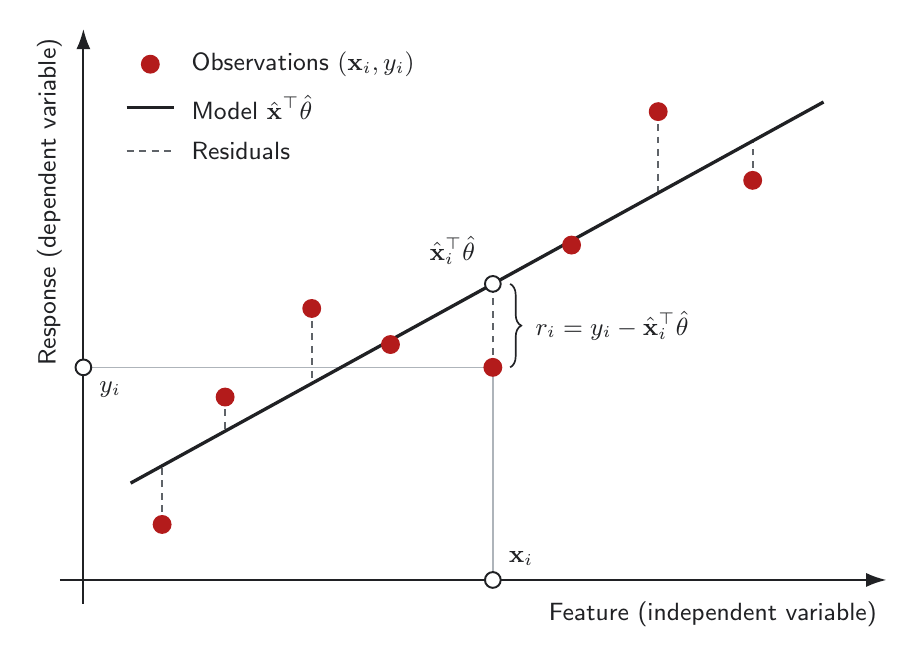
\begin{tikzpicture}[x=1cm, y=1cm, font=\sffamily\small, text=vnink,
    axis/.style={draw=vnink, line width=0.8pt, -{Latex[length=2.6mm, width=1.8mm]}},
    model/.style={draw=vnink, line width=1.2pt},
    residual/.style={draw=vnmuted, line width=0.8pt, dash pattern=on 2.5pt off 2pt},
    guide/.style={draw=vnrule, line width=0.5pt},
    obs/.style={circle, fill=vncarnelian, draw=none, inner sep=0pt, minimum size=2.4mm},
    open/.style={circle, fill=white, draw=vnink, line width=0.7pt, inner sep=0pt, minimum size=2mm},
  ]
  % fitted line y = a + b x
  \pgfmathsetmacro{\intercept}{0.9}
  \pgfmathsetmacro{\slope}{0.55}

  % observation i, highlighted with guides to both axes
  \pgfmathsetmacro{\xobs}{5.2}
  \pgfmathsetmacro{\yobs}{2.7}
  \pgfmathsetmacro{\yfit}{\intercept + \slope*\xobs}

  % guides first, so the axes, line, and markers draw over them
  \draw[guide] (0, \yobs) -- (\xobs, \yobs);
  \draw[guide] (\xobs, 0) -- (\xobs, \yobs);

  % axes
  \draw[axis] (-0.3, 0) -- (10.2, 0);
  \draw[axis] (0, -0.3) -- (0, 7.0);
  \node[anchor=north east] at (10.2, -0.15) {Feature (independent variable)};
  \node[rotate=90, anchor=south east] at (-0.15, 7.0) {Response (dependent variable)};

  % residuals: dashed from each observation to the line
  \foreach \x/\y in {1/0.705, 1.8/2.323, 2.9/3.448, 3.9/2.99, 6.2/4.253, 7.3/5.948, 8.5/5.075} {
    \draw[residual] (\x, \y) -- (\x, {\intercept + \slope*\x});
  }
  \draw[residual] (\xobs, \yobs) -- (\xobs, \yfit);

  % model line
  \draw[model] (0.6, {\intercept + \slope*0.6}) -- (9.4, {\intercept + \slope*9.4});

  % observations
  \foreach \x/\y in {1/0.705, 1.8/2.323, 2.9/3.448, 3.9/2.99, 6.2/4.253, 7.3/5.948, 8.5/5.075} {
    \node[obs] at (\x, \y) {};
  }
  \node[obs] at (\xobs, \yobs) {};

  % observation i: axis markers, fitted value, and residual brace
  \node[open] at (\xobs, 0) {};
  \node[open] at (0, \yobs) {};
  \node[anchor=south west] at ({\xobs + 0.08}, 0.06) {$\mathbf{x}_{i}$};
  \node[anchor=north west] at (0.08, {\yobs - 0.06}) {$y_{i}$};
  \node[open] at (\xobs, \yfit) {};
  \node[anchor=south east] at ({\xobs - 0.1}, {\yfit + 0.12}) {$\hat{\mathbf{x}}_{i}^{\top}\hat{\mathbf{\theta}}$};
  \draw[vnink, line width=0.6pt, decorate, decoration={brace, amplitude=4pt, mirror}]
    ({\xobs + 0.22}, \yobs) -- ({\xobs + 0.22}, \yfit);
  \node[anchor=west] at ({\xobs + 0.42}, {(\yobs + \yfit)/2})
    {$r_{i} = y_{i} - \hat{\mathbf{x}}_{i}^{\top}\hat{\mathbf{\theta}}$};

  % legend
  \node[obs] at (0.85, 6.55) {};
  \node[anchor=west] at (1.25, 6.55) {Observations $(\mathbf{x}_{i}, y_{i})$};
  \draw[model] (0.55, 6.0) -- (1.15, 6.0);
  \node[anchor=west] at (1.25, 6.0) {Model $\hat{\mathbf{x}}^{\top}\hat{\mathbf{\theta}}$};
  \draw[residual] (0.55, 5.45) -- (1.15, 5.45);
  \node[anchor=west] at (1.25, 5.45) {Residuals};
\end{tikzpicture}
\end{document}
